Dans cette section, nous allons détailler le processus complet de génération d'un projet de travail pour CROCO en utilisant l'interface QCrocoFlow. L'objectif est de fournir une vue d'ensemble claire et concise des différentes étapes nécessaires pour passer de la phase initiale à l'obtention de tous les fichiers requis pour une simulation CROCO. Cette démarche permet non seulement de garantir la cohérence et la précision des données utilisées, mais aussi de faciliter la reproductibilité des simulations pour d'autres utilisateurs ou d'autres études. 

Nous allons parcourir chaque étape, en mettant l'accent sur les choix clés effectués, les outils utilisés et les résultats obtenus à chaque phase. Cette approche pas à pas permettra d'appréhender l'efficacité et la simplicité du processus, tout en mettant en évidence la robustesse et la flexibilité de l'outil QCrocoFow dans la gestion des projets CROCO.

\subsection{Paramètres utilisateurs de la zone}

Nous illustrons ici le processus de création d'une configuration pour la zone de Saint-Vaast-la-Hougue, située en Normandie. La simulation est prévue pour la période du 1er janvier 2016 au 1er février 2016. 

\begin{enumerate}
	\item \textbf{Sélection du chemin de sortie :} La première étape consiste à définir un dossier de sortie où tous les fichiers générés seront stockés. Un dossier nommé \texttt{"SntVast"} a été créé à cet effet.
	\begin{figure}[h]
		\centering
			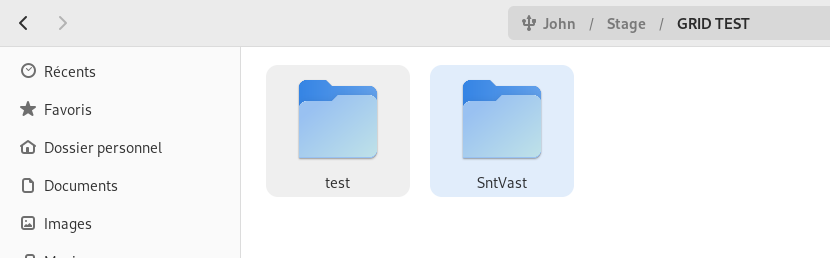
\includegraphics[width=0.6\textwidth]{./IMAGES/resultats/chemin_sortie.png}
		\caption{Dossier de sortie nommé \texttt{"SntVast"}.}
		\label{fig:chemin_sortie}
	\end{figure}
	
	\item \textbf{Titre et nom de la grille :} Pour cette simulation, le titre et le nom de la grille ont été définis comme \texttt{"SntVast"}.
	
	\item \textbf{Choix de la période de simulation :} La période sélectionnée s'étend du 1er janvier 2016 au 1er février 2016.
	
	\item \textbf{Sélection du fichier topographique :} Le fichier topographique utilisé pour cette simulation provient du site du SHOM et est nommé \texttt{MNT\_ATL100m}.
	
	\newpage
	\begin{figure}[h]
		\centering
		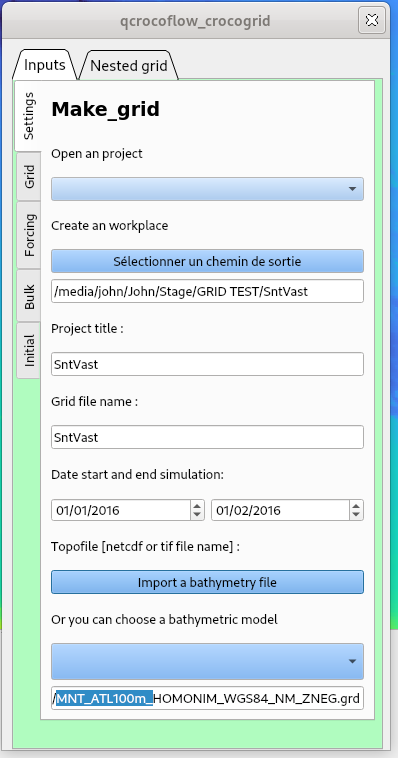
\includegraphics[width=0.5\textwidth]{./IMAGES/resultats/qcroco_param.png}
		\caption{Interface QCrocoFlow montrant les paramètres sélectionnés pour la simulation.}
		\label{fig:qcroco_param}
	\end{figure}
\end{enumerate}

Ces étapes initiales permettent de définir les paramètres de base nécessaires à la création d'une configuration CROCO adaptée à la zone d'étude choisie.

\subsection{Choix de la zone d'étude et génération du fichier \texttt{grid}}

La définition précise de la zone d'étude est cruciale pour obtenir des résultats de simulation pertinents. Voici les étapes suivies pour définir la zone d'étude et générer le fichier \texttt{grid} :

\begin{enumerate}
	\item \textbf{Choix de la résolution des mailles :} Pour cette simulation, une résolution de 500 mètres a été choisie pour les mailles.
	
	\item \textbf{Sélection de la zone de travail :} La zone de Saint-Vaast-la-Hougue a été sélectionnée directement sur la carte intégrée à l'interface Qcrocoflow. Les coordonnées de cette zone sont automatiquement affichées dans l'interface.
	
	\item \textbf{Sauvegarde des paramètres :} Cette fonctionnalité permet de sauvegarder les paramètres de la simulation. C'est particulièrement utile si l'on envisage de réaliser plusieurs simulations dans la même zone ou si l'on souhaite apporter des modifications ultérieures à la configuration.
	
	\item \textbf{Lancement de la génération :} Après avoir défini tous les paramètres, le bouton \textit{Process} est utilisé pour lancer la génération du fichier \texttt{grid}.
	\begin{figure}[h]
		\centering
		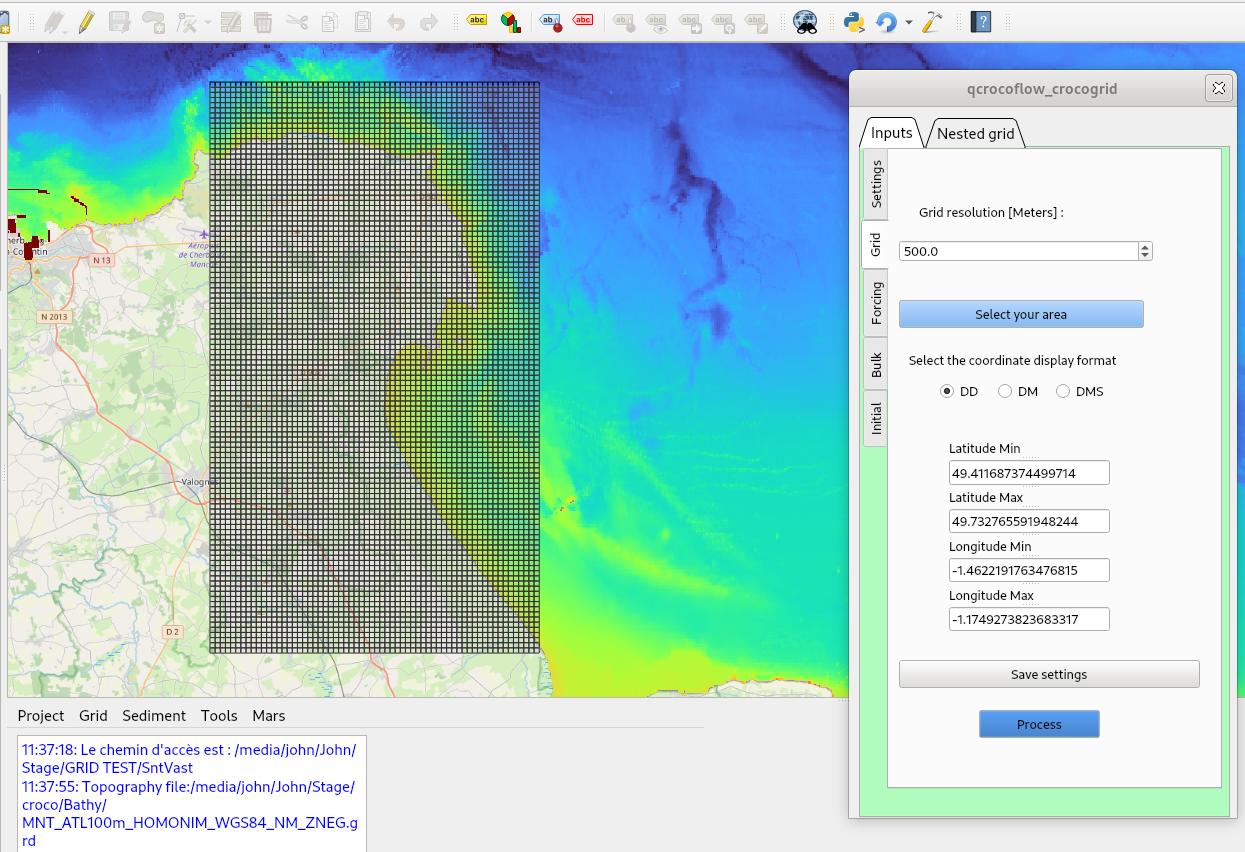
\includegraphics[width=0.7\textwidth]{./IMAGES/resultats/qcroco_grid.png}
		\caption{Paramètres de la grille dans Qcrocoflow avec visualisation de la zone d'étude sur la carte.}
		\label{fig:qcroco_grid}
	\end{figure}
\end{enumerate}

Après avoir suivi les étapes précédentes, le fichier \texttt{grid} destiné à CROCO est généré. Ce fichier contient toutes les informations nécessaires concernant la grille de simulation, y compris la topographie, la résolution des mailles, et les coordonnées de la zone d'étude.

\begin{figure}[h]
	\centering
	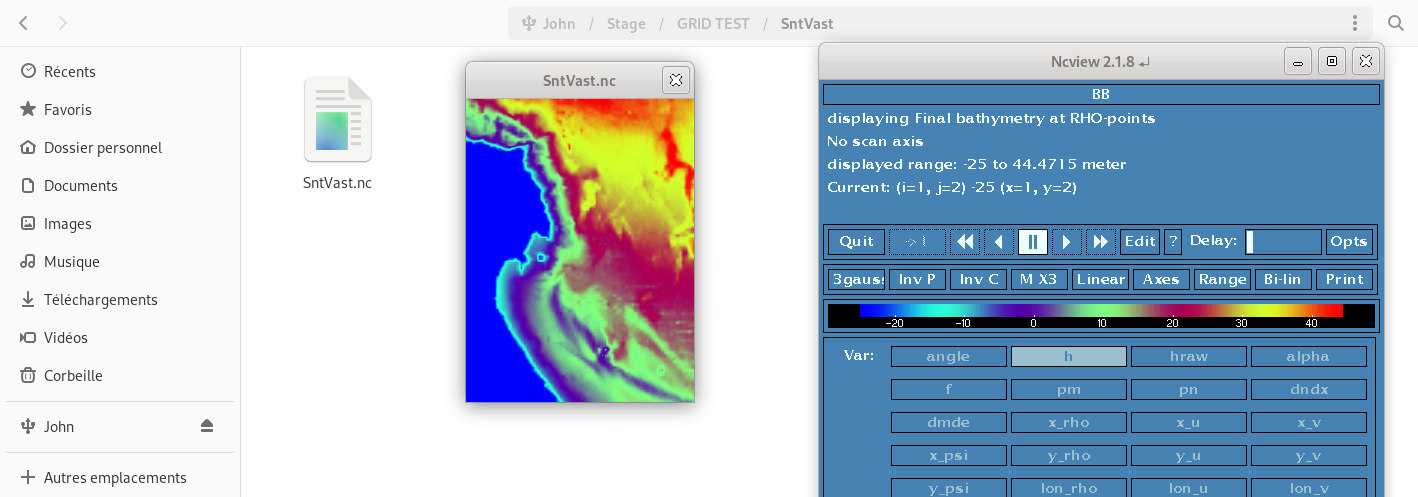
\includegraphics[width=0.7\textwidth]{./IMAGES/resultats/SntVast_grd.png}
	\caption{Aperçu du fichier \texttt{SntVast.grd} généré pour la simulation.}
	\label{fig:gdr_croco}
\end{figure}

La figure \ref{fig:gdr_croco} montre un aperçu du fichier généré. Avec ce fichier en place, nous sommes maintenant prêts à procéder aux étapes suivantes de la configuration de la simulation dans CROCO.

\subsection{Génération des fichiers de forçage par marées}

Pour générer les fichiers de forçage par marées, il est impératif d'avoir préalablement obtenu l'accès au modèle TPXO9, comme détaillé dans le chapitre précédent.

\begin{enumerate}
	\item \textbf{Sélection du dossier TPXO9} : Dans cette étape, l'utilisateur doit indiquer le chemin vers le dossier contenant le modèle de marée TPXO9.
	
	\item \textbf{Choix des harmoniques de marée} : L'utilisateur a la possibilité de sélectionner les harmoniques de marée qu'il souhaite utiliser pour la simulation CROCO. Pour notre étude, nous avons choisi de conserver toutes les harmoniques par défaut afin d'obtenir une résolution optimale du modèle CROCO.
	
	\item \textbf{Lancement de la génération} : Une fois les étapes précédentes complétées, il suffit de cliquer sur le bouton "Process" pour lancer la génération des fichiers de forçage.
\end{enumerate}

\begin{figure}[h]
	\centering
	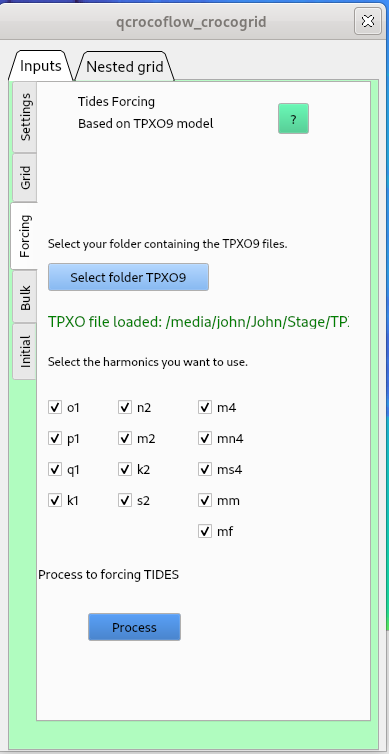
\includegraphics[width=0.4\textwidth]{./IMAGES/resultats/Qcrocoflow_Forcing.png}
	\caption{Interface Qcrocoflow pour la génération des fichiers de forçage par marées.}
	\label{fig:qcroco_forcing}
\end{figure}

La figure \ref{fig:qcroco_forcing} illustre l'interface Qcrocoflow dédiée à la génération des fichiers de forçage par marées.\\

Suite aux étapes précédemment décrites, le fichier de forçage pour la zone de Saint-Vaast-la-Hougue a été généré et est prêt à être utilisé dans CROCO. Ce fichier, nommé \texttt{SntVast\_frc01Jan2016.nc}, est nommé en fonction du nom de la grille et de la date de début de la simulation.La figure \ref{fig:sntvast_forcing} montre un aperçu du fichier de forçage généré pour la zone de Saint-Vaast-la-Hougue.


\begin{figure}[h]
	\centering
	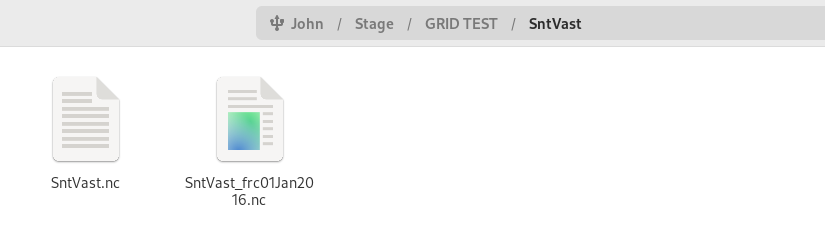
\includegraphics[width=0.7\textwidth]{./IMAGES/resultats/SntVast_ForcingFile.png}
	\caption{Aperçu du fichier de forçage \texttt{SntVast\_frc01Jan2016.nc} pour la zone de Saint-Vaast-la-Hougue.}
	\label{fig:sntvast_forcing}
\end{figure}

\subsection{Génération des fichiers météorologiques : BULK}

Pour la génération des fichiers météorologiques, il est impératif d'avoir préalablement créé un compte sur le site ERA5 et d'avoir le fichier contenant les informations de connexion, comme mentionné dans le chapitre dédié.

\paragraph{Étape 1 : Téléchargement des données ERA5}
Si aucune donnée pour la zone n'a été téléchargée au préalable, cette étape va créer un dossier \texttt{BULK\_FILE} qui contiendra deux sous-dossiers : \texttt{ERA5\_native\_"nom du projet"} et \texttt{ERA5\_"nom du projet"}. Le premier contient les fichiers météorologiques bruts, tandis que le second contient les fichiers météorologiques convertis pour la suite du script.

\begin{figure}[h]
	\centering
	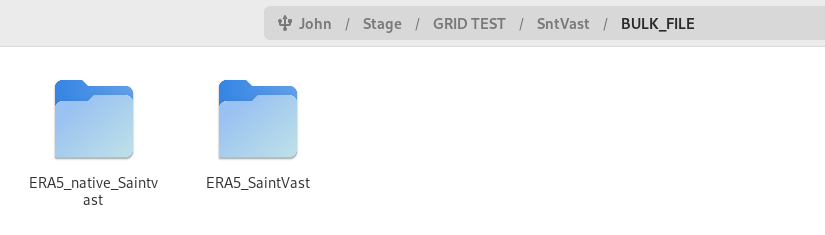
\includegraphics[width=0.7\textwidth]{./IMAGES/resultats/BulkFiles.png}
	\caption{Aperçu des dossiers générés après le téléchargement des données ERA5.}
	\label{fig:bulk_files}
\end{figure}

Il est important de noter que si les données ont déjà été téléchargées pour la zone, il suffira de sélectionner le dossier \texttt{ERA5\_SaintVast} plutôt que de télécharger à nouveau les données.

\paragraph{Étape 2 : Génération des fichiers BULK}
En cliquant sur "Process", la génération des fichiers BULK est lancée.
\newpage
\begin{figure}[h]
	\centering
	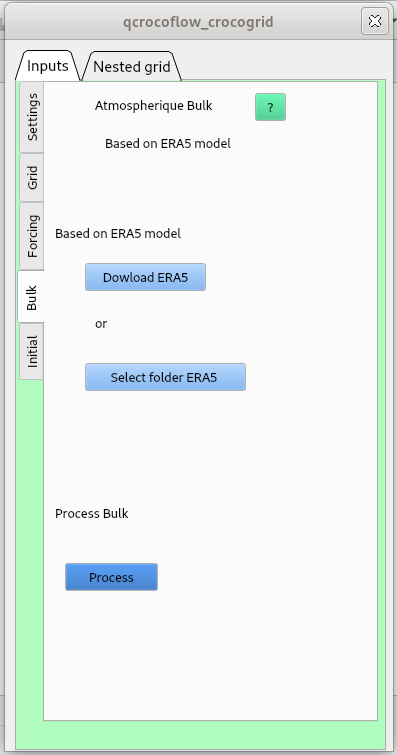
\includegraphics[width=0.2\textwidth]{./IMAGES/resultats/Qcroco_Bulk.png}
	\caption{Interface QCrocoFlow pour la génération des fichiers BULK.}
	\label{fig:qcroco_bulk}
\end{figure}

À la fin de cette étape, les fichiers météorologiques (BULK) sont générés dans le dossier de travail et sont prêts à être incorporés dans le modèle CROCO. Pour notre simulation du 1/1/2016 au 1/2/2016, deux fichiers sont générés pour chaque mois. Ils sont nommés : \texttt{SntVast\_bulkY2016M01}, correspondant au titre de la grille, à l'année et au mois de la simulation.


\begin{figure}[h]
	\centering
	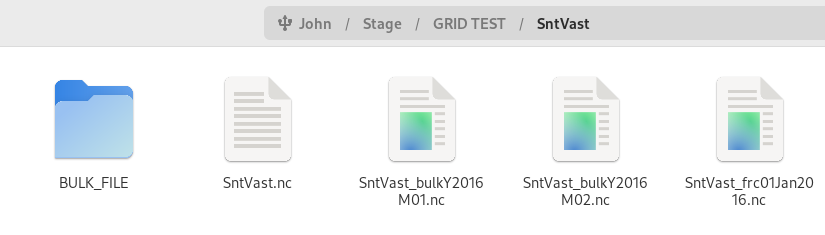
\includegraphics[width=0.7\textwidth]{./IMAGES/resultats/BulkGeneratedFiles.png}
	\caption{Fichiers BULK générés pour la simulation.}
	\label{fig:bulk_generated}
\end{figure}


\subsection{Conclusion de la configuration CROCO pour Saint-Vast-la-Hougue}

La configuration de CROCO pour la zone de Saint-Vast-la-Hougue a été réalisée en moins de cinq minutes, démontrant ainsi l'efficacité et la rapidité de l'outil QCrocoFlow. Bien que la paramétrisation et le lancement de la simulation CROCO ne soient pas directement liés au contexte de mon stage, il était essentiel de vérifier la validité des fichiers générés.

Pour ce faire, plusieurs simulations ont été lancées dans différentes zones. Les résultats ont été concluants, attestant que les fichiers générés sont non seulement fonctionnels, mais également bien paramétrés. Cela confirme la robustesse de l'outil développé et sa capacité à fournir des configurations prêtes à l'emploi pour CROCO.
